\begin{figure}
  \setlength{\unitlength}{\textwidth}
  \fbox{
  \begin{picture}(1,0.4)(0,0.8)
    
    % % %90
      \put(0.025,0.9){\includegraphics[width=0.5\unitlength]{../FnP/gnuplot/vel_time_history_60_0.075.eps}}
      \put(0.495,0.9){\includegraphics[width=0.5\unitlength]{../FnP/gnuplot/vel_time_history_165_0.175.eps}}
     
   
	
            
      
      
   
 	\put(-0.01,1.02){ $\frac{V}{D}$} 	
% 	\put(0.56,1.02){ $\frac{V}{D}$}
 	
 	 	\put(0.25,0.88){ $\frac{tU}{D}$} 	
 	 	\put(0.73,0.88){ $\frac{tU}{D}$}



    \put(0.095,1.1){(a)}
    \put(0.565,1.1){(b)}
   
       

  \end{picture}
}
  \caption{Time histories of velocity at two different $\zeta$ and $U^*$ which produces same mean power ($1.2\times10^{-3}$). Data presented using QSS assumption, (a) at \ustar=60 and $\zeta=0.075$, (b) at \ustar=165 and $\zeta=0.175$ at Re=165. Shedding is present in both signals as noise but the average velocity amplitude remain constant in both cases.}
    \label{fig:time_hostory_velocity_same_power}
\end{figure}